\documentclass[a4]{article}

\usepackage[left=2cm,right=2cm,top=2cm,bottom=2cm]{geometry} 

\usepackage[utf8]{inputenc}   % otra alternativa para los caracteres acentuados y la "ñ"
\usepackage[           spanish % para poder usar el español
                      ,es-tabla % para los captions de las tablas
                       ]{babel}   
\decimalpoint %para usar el punto decimal en vez de coma para los números con decimales

\usepackage{beton}
\usepackage[T1]{fontenc}

\usepackage{parskip}
\usepackage{xcolor}

\usepackage{caption}

\usepackage{enumerate} % paquete para poder personalizar fácilmente la apariencia de las listas enumerativas

\usepackage{graphicx} % figuras
\usepackage{subfigure} % subfiguras

\usepackage{amsfonts}
\usepackage{amsmath}

\definecolor{gris}{RGB}{220,220,220}
	
\usepackage{float} % para controlar la situación de los entornos flotantes

\restylefloat{figure}
\restylefloat{table} 
\setlength{\parindent}{0mm}


\usepackage[bookmarks=true,
            bookmarksnumbered=false, % true means bookmarks in 
                                     % left window are numbered                         
            bookmarksopen=false,     % true means only level 1
                                     % are displayed.
            colorlinks=true,
            allcolors=blue]{hyperref}
\definecolor{webblue}{rgb}{0, 0, 0.5}  % less intense blue


\title{AA: Práctica 3}

\author{David Cabezas Berrido}

\date{}

\begin{document}

\maketitle
\tableofcontents

\newpage

\section{Clasificación de dígitos manuscritos}

\subsection{Problema}

Se nos pide clasificar imágenes de dígitos escritos a mano para
reconocer el dígito que representan (del 0 al 9). Disponemos de
ejemplos clasificados para aprender, por lo que podemos enfocarlo como
un problema de aprendizaje supervisado. Concretamente se trata de un
problema de clasificación en el que tenemos 10 clases, los dígitos del
0 al 9.

En el archivo \texttt{opdigits.names} encontramos información sobre
los datos que nos proporcionan. Constan de un conjunto con 3823
instancias para training y 1791 para test, cada instancia tiene 64
atributos que representan el número de bits coloreados (entre 0 y 16)
en cada una de las 64 casillas que forman una cuadrícula de
$8\times 8$.

Podemos visualizar ĺas instancias como matrices en lugar de vectores
para comprender mejor el formato de los datos.

\vspace{-5mm}
\begin{figure}[H]
  \centering
  \subfigure[Instancia correspondiente al 0]{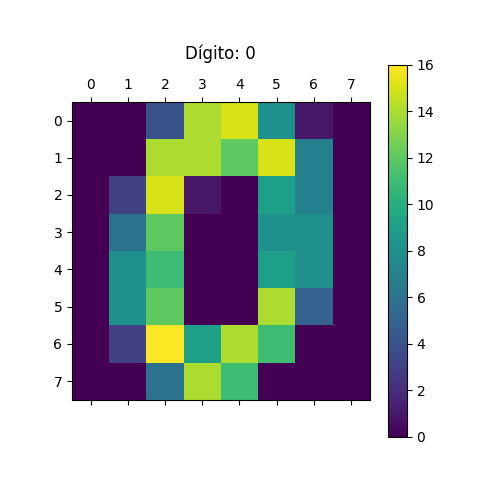
\includegraphics[width=57.5mm]{imgs/sample1.png}}
  \subfigure[Instancia correspondiente al 9]{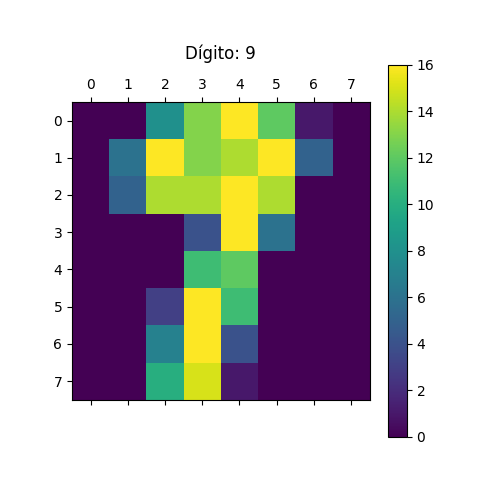
\includegraphics[width=57.5mm]{imgs/sample2.png}}
  \subfigure[Instancia correspondiente al 8]{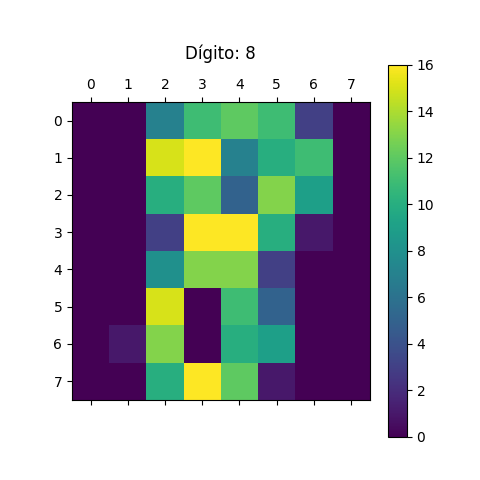
\includegraphics[width=57.5mm]{imgs/sample3.png}}
  \caption{Algunas instancias de los datos}
  \label{fig:digits-matrix}
\end{figure}

La población $X$ constituye el conjunto de vectores de 64 enteros
entre 0 y 16 que representan la cuadricula resultante de aplicar la
trasformación antes comentada; el conjunto de clases $Y$ constituye
los posibles dígitos: 0,1,2,3,4,5,6,7,8,9; y la función objetivo $f$
es la que asigna a cada vector de $X$ la clase del dígito que
representa.

Cabe preguntarnos si con los datos que tenemos podemos entrenar un
buen modelo, pues se ha perdido parte de la información al agrupar los
bits por cuadrículas. Para ello, podemos usar la función PCA
(Principal Component Analysis) para proyectar las dos características
que más me ayudan a distinguir los datos. Luego partimos de esa
proyección y aplicamos algoritmo TSNE (T-distributed Stochastic
Neighbor Embedding) para proyectar los datos en dos dimensiones de
forma que para cada dato sus vecinos más cercanos queden proyectados
cerca. Ambos algoritmos se encuentran progamados en \textit{sklearn}.

\begin{figure}[H]
  \centering
  \subfigure[Proyección 2D mediante PCA]{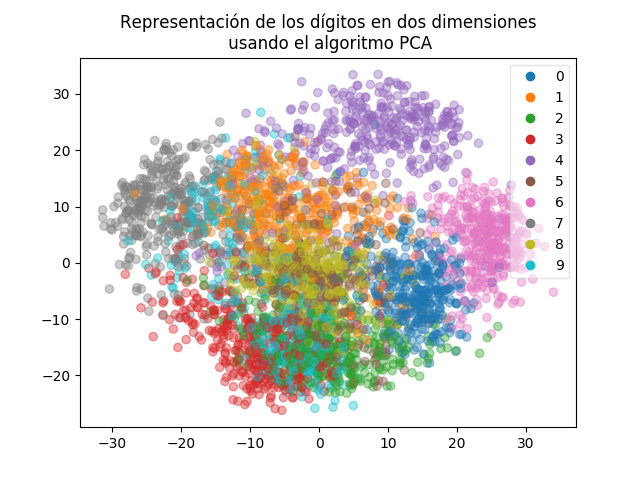
\includegraphics[width=87mm]{imgs/2dPCA.png}}
  \subfigure[Proyección 2D mediante T-SNE]{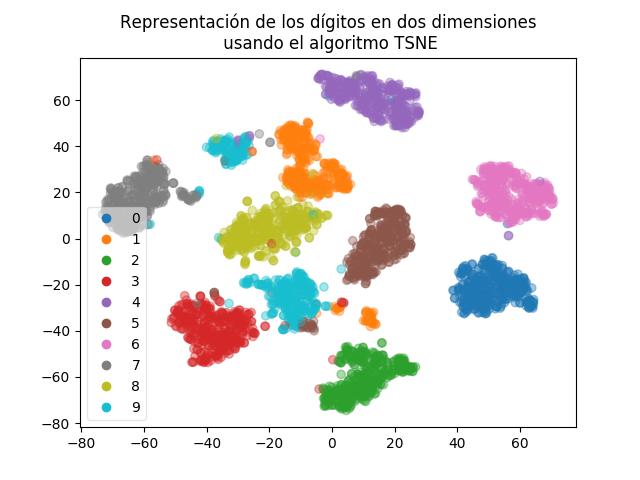
\includegraphics[width=87mm]{imgs/2dTSNE.png}}
  \caption{Visualización en 2D de los datos}
  \label{fig:2D-projection}
\end{figure}
\vspace{-4mm}

Sólo con las características principales ya podemos discernir
ligeramente entre los datos de diferentes clases. Y si tenemos en
cuenta todas ellas, los dígitos correspondientes a la misma clase se
encuentran bastante agrupados exceptuando algunas instancias sueltas.


\subsection{Conjuntos de training y test}

Los datos que nos proporcionan vienen ya separados en conjuntos de
training y test, y es importante que mantengamos esta división.

El motivo es que los datos de training corresponden a dígitos hechos a
mano por 30 personas diferentes y los datos de test a los de otras 13
personas.

Siempre es importante que en training y en test se utilicen conjuntos
disjuntos de datos para que $E_{test}$ sea un estimador de $E_{out}$
lo más representativo posible. Pero además en este problema es
importante que los dígitos usados en test estén hechos por personas
diferentes a las que generaron los dígitos de train, ya que es
presumible que el modelo reconozca mejor los dígitos trazados por las
mismas personas que trazaron los dígitos de entrenamiento.

Este hecho provoca que la estimación de $E_{out}$ realizada con
Cross-Validation sea demasiado optimista, por ser los datos de
validación correspondientes a las mismas personas que los de
entrenamiento.


\subsection{Clases de funciones a usar y Preprocesamiento}

La clase de funciones que usaremos son los polinomios de grado 2, ya
que permiten obtener un modelo mucho más complejo y potente que
utilizar simplemente características lineales. Para añadir
características polinomiales usamos PolynomialFeatures.

El motivo por el que presento esta sección junto con procesamiento es
que la introducción de características polinomiales eleva el número de
variables al grado del polinomio, esto es computacionalmente costoso y
provoca que acabemos con demasiadas características. De hecho,
introducir características polinómicas de grado mayor que 2 es ya
demasiado costoso, por lo que no usamos grados más altos. Por este
motivo he decidido añadir la indroducción de características
polinomiales al preprocesamiento.

Para el preprocesamiento, creamos un Pipeline que primero elimina con
Variance Threshold las características con varianza menor que un
umbral, en mi caso 0.005. Estas características apenas ayudan a
distinguir las instancias de la muestra. En segundo lugar añade
características de grado 2, ahora el número de características es
igual al cuadrado de las que quedaban tras la primera selección en
lugar de $64^2$. A continuación, realiza una estandarización con
StandardScaler y escala las variables para dejar todas con media 0 y
varianza 1. Por último utiliza otra vez PCA, pero esta vez en lugar de
proyectar un número fijo de variables, selecciona el menor número
posible que expliquen cierto porcentaje de la variabilidad de la
muestra, en este caso un 97.5\%.

Ajustamos el Pipeline con los datos de train y aplicamos las
transformaciones tanto a los de train como a los de test. Partíamos de
64 características y nos quedamos con 312. Teniendo en cuenta que
$64^2=4096$, sacrificando un pequeño porcentaje de la información
nos quedamos con un conjunto de variables bastante manejable.

Tanto el objeto Pipeline como los que realizan cada paso del
preprocesado se encuentran en \textit{sklearn}.

Para apreciar el resultado del preprocesado podemos visualizar la
matriz de coeficientes de correlación de Pearson, que indica la medida
en que unas características determinan otras. Si una característica
está determinada por el resto, se podría eliminar sin perder
información. Por tanto interesa que esta matriz sea diagonal, que cada
variable se determine únicamente a ella misma.

\vspace{-4mm}
\begin{figure}[H]
  \centering
  \subfigure[Antes del preprocesado]{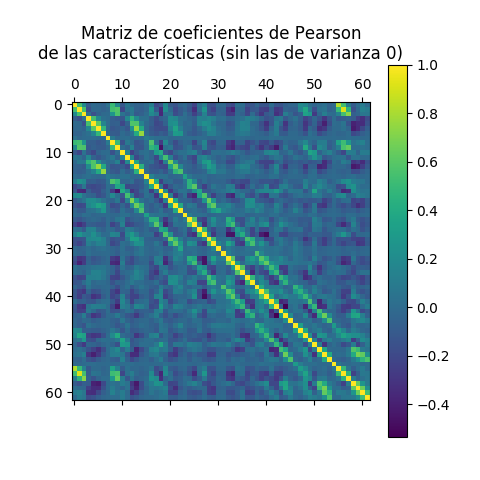
\includegraphics[width=87mm]{imgs/pearsonRaw.png}}
  \subfigure[Después del preprocesado]{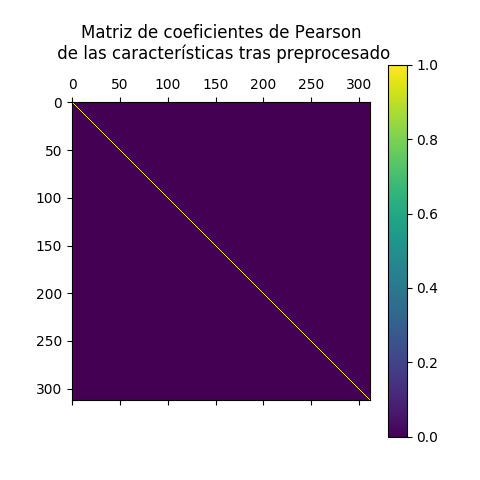
\includegraphics[width=87mm]{imgs/pearsonPre.png}}
  \caption{Matrices de coeficientes de correlación de Pearson}
  \label{fig:pearson}
\end{figure}
\vspace{-4mm}

Como podemos ver, fuera de la diagonal todos los coeficientes son
practicamente 0 como queríamos.

\subsection{Métricas}



\subsection{Ajuste del modelo}

\subsection{Regularización}

\subsection{Modelos}

\subsection{Estimación de hiperparámetros y selección del modelo}

\subsection{Estimación de $E_{out}$}

\subsection{Conclusiones}

\end{document}
